\section{Evaluation}
In this section we will now make use of the previous sections: Forwarding the channel to the time regime and
reducing the background from our main figure in order to evaluate the half life period.
\subsection{Naive approach: Ad-hoc solution}
The measurement of randomized concidences lasted 4.1 lasted \textbf{6080 seconds} = 1 hour 41 minutes and 20 seconds, while
the measurement of delayed coincidences lasted \textbf{52658 seconds} =  14 hours, 37 minutes and 38 seconds. 
In order to compensate for this disparity, we need to extrapolate the background by the following
\begin{equation}
\mathrm{\textbf{total:} } \quad 79 \quad \mathrm{events} \quad \Rightarrow 5.177\cdot 10^{-5}\quad \mathrm{events/ (channel \cdot second)}
\end{equation}
If we extrapolate this for the delayed coincidences, we arrive at
\begin{align}
\begin{split}
\mathrm{\textbf{background estimate:} } \quad  5.177\cdot 10^{-5} \cdot 52658 \quad \mathrm{events / channel} \\
= 2.726\quad \mathrm{events/ channel}
\end{split}
\end{align}
Now we 

\begin{figure}[htpb]
    \centering
    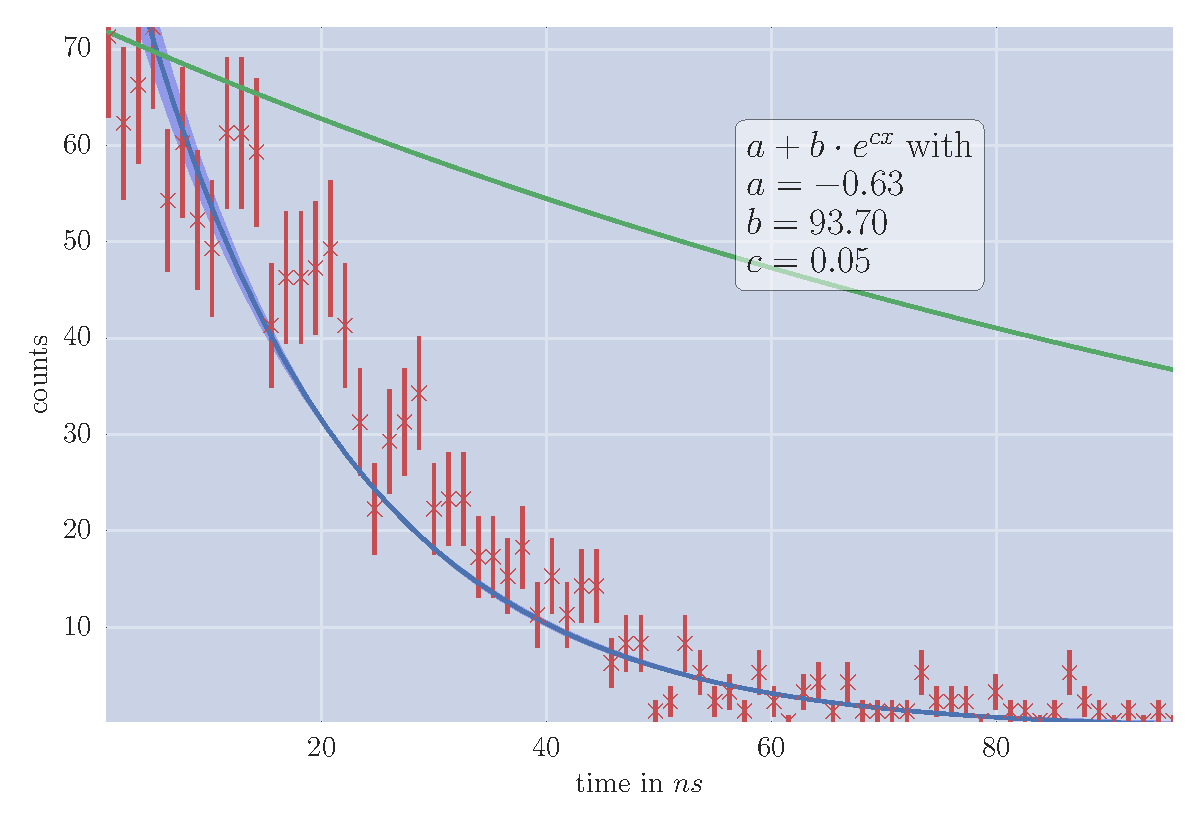
\includegraphics[width=0.8\linewidth]{analysis/figures/plot4_1_reg}
    \caption{Name}
    \label{fig:name}
\end{figure}




